% Created 2022-01-17 Mon 01:46
% Intended LaTeX compiler: pdflatex
\documentclass[11pt]{article}
\usepackage[hidelinks]{hyperref}
\usepackage[utf8]{inputenc}
\usepackage[T1]{fontenc}
\usepackage{graphicx}
\usepackage{longtable}
\usepackage{wrapfig}
\usepackage{rotating}
\usepackage[normalem]{ulem}
\usepackage{amsmath}
\usepackage{amssymb}
\usepackage{capt-of}
\usepackage{hyperref}
\usepackage{parskip}
\usepackage{siunitx}
\usepackage{svg}
\usepackage{minted}
\usepackage[margin=1in]{geometry}
\definecolor{bg}{rgb}{0.95,0.95,0.95}
\setminted{frame=single,bgcolor=bg,samepage=true}
\setlength{\parindent}{0pt}
\sisetup{per-mode=fraction}
\usepackage[shellescape]{gmp}
\usepackage{gauss}
\usepackage{float}
\usepackage[inkscapearea=page/nocrop]{svg}
\usepackage{cancel}
\usepackage{amssymb}
\usepackage{titlesec}
\usepackage{mathtools, nccmath}
\newcommand{\Lwrap}[1]{\left\{#1\right\}}
\newcommand{\Lagr}[1]{\mathcal{L}\Lwrap{#1}}
\newcommand{\Lagri}[1]{\mathcal{L}^{-1}\Lwrap{#1}}
\newcommand{\Ztrans}[1]{\mathcal{Z}\Lwrap{#1}}
\newcommand{\Ztransi}[1]{\mathcal{Z}^{-1}\Lwrap{#1}}
\newcommand{\ZOH}[1]{\text{ZOH}\left(#1\right)}
\DeclarePairedDelimiter{\ceil}{\lceil}{\rceil}
\makeatletter \AtBeginEnvironment{minted}{\dontdofcolorbox} \def\dontdofcolorbox{\renewcommand\fcolorbox[4][]{##4}} \makeatother
\titleformat{\paragraph}[hang]{\normalfont\normalsize\bfseries}{\theparagraph}{1em}{}
\titlespacing*{\paragraph}{0pt}{3.25ex plus 1ex minus .2ex}{0.5em}
\setcounter{secnumdepth}{5}
\author{Jasper Chan - 37467164 \\ jasperchan515@gmail.com}
\date{\today}
\title{MECH 464 Homework Assignment 1}
\hypersetup{
 pdfauthor={Jasper Chan - 37467164 \\ jasperchan515@gmail.com},
 pdftitle={MECH 464 Homework Assignment 1},
 pdfkeywords={},
 pdfsubject={},
 pdfcreator={Emacs 27.2 (Org mode 9.5.2)}, 
 pdflang={English}}
\begin{document}

\maketitle


\section{Exercise 1}
\label{sec:org54fd893}
Find, by hand, the eigenvalues and eigenvectors of \(A\) as well as \(e^{At}\) for

\begin{equation*}
A = 
\begin{bmatrix}
0      & -\omega & 0 \\
\omega & 0       & 0 \\
0      & 0       & 0
\end{bmatrix}
\end{equation*}

\subsection{Solution}
\label{sec:orgd5f8a0d}
\subsubsection{Eigenvalues and Eivenvectors}
\label{sec:org8ecda6d}
Let's find the eigenvalues \(\lambda\) by solving \(|A - \lambda \mathbf{I}| = 0\)

\begin{align*}
0 &= |A - \lambda \mathbf{I}| \\
&=
\begin{vmatrix}
-\lambda & -\omega  & 0 \\
\omega   & -\lambda & 0 \\
0        & 0        & -\lambda
\end{vmatrix} \\
&=
\left[
    (-\lambda)(-\lambda)(-\lambda)
    + (-\omega)(0)(0)
    + (0)(\omega)(0)
\right]
-
\left[
    (0)(-\lambda)(0)
    + (-\lambda)(0)(0)
    + (-\omega)(\omega)(-\lambda)
\right] \\
&=
\left[
    -\lambda^3
\right]
-
\left[
    \lambda\omega^2
\right] \\
&=
-\lambda\left(\lambda^2 + \omega^2\right)
\end{align*}
The eigenvalues are then:
\begin{align*}
\lambda_1 &= 0 &
\lambda_2 &= -\omega j &
\lambda_3 &= \omega j
\end{align*}

Now we can use row reduction to solve for each eigenvector

\paragraph{\(\lambda_1 = 0\)}
\label{sec:org26ba1fd}
\begin{align*}
A - \lambda_1\mathbf{I} &= A \\
&=
\begin{gmatrix}[b]
0      & -\omega & 0 \\
\omega & 0       & 0 \\
0      & 0       & 0
\rowops
  \mult{0}{/-\omega}
  \mult{1}{/\omega}
\end{gmatrix}
\Rightarrow
\begin{gmatrix}[b]
0 & 1 & 0 \\
1 & 0 & 0 \\
0 & 0 & 0
\end{gmatrix}
\end{align*}

\begin{align*}
a_{e_1} &= 0 &
b_{e_1} &= 0 &
c_{e_1} &= 1 \\
&&
\underbar{e}_1 &=
\begin{bmatrix}
0 \\ 0 \\ 1
\end{bmatrix}
\end{align*}
\paragraph{\(\lambda_2 = -\omega j\)}
\label{sec:orge9b4620}
\begin{align*}
A - \lambda_2\mathbf{I}
&=
\begin{gmatrix}[b]
\omega j & -\omega  & 0 \\
\omega   & \omega j & 0 \\
0        & 0        & \omega j
\rowops
  \mult{0}{/\omega}
  \mult{1}{/\omega}
  \mult{2}{/\omega j}
  \mult{0}{\cdot j}
  \add[1]{1}{0}
\end{gmatrix}
\Rightarrow
\begin{gmatrix}[b]
0 & 0 & 0 \\
1 & j & 0 \\
0 & 0 & 1
\end{gmatrix}
\end{align*}

\begin{align*}
a_{e_2} &= -j &
b_{e_2} &= 1 &
c_{e_2} &= 0 \\
&&
\underbar{e}_2 &=
\begin{bmatrix}
-j \\ 1 \\ 0
\end{bmatrix}
\end{align*}

\paragraph{\(\lambda_3 = \omega j\)}
\label{sec:org72d533c}

We know the third eigenvector should be the complex conjugate of the second, however let's prove this:

\begin{align*}
A - \lambda_3\mathbf{I}
&=
\begin{gmatrix}[b]
-\omega j & -\omega   & 0 \\
 \omega   & -\omega j & 0 \\
 0        & 0         & -\omega j
\rowops
  \mult{0}{/-\omega}
  \mult{1}{/\omega}
  \mult{2}{/-\omega j}
  \mult{1}{\cdot j}
  \add[-1]{0}{1}
\end{gmatrix}
\Rightarrow
\begin{gmatrix}[b]
j & 1 & 0 \\
0 & 0 & 0 \\
0 & 0 & 1
\end{gmatrix}
\end{align*}

\begin{align*}
a_{e_3} &= j &
b_{e_3} &= 1 &
c_{e_3} &= 0 \\
&&
\underbar{e}_3 &=
\begin{bmatrix}
j \\ 1 \\ 0
\end{bmatrix}
\end{align*}

\paragraph{Answer Checking}
\label{sec:org5581f19}
Using MATLAB to check our work:

\begin{minted}[]{matlab}
syms omega t;
A = [0 -omega 0; omega 0 0; 0 0 0]
[e, lambda] = eig(A)
\end{minted}

\begin{minted}[]{matlab}
A =
 
[    0, -omega, 0]
[omega,      0, 0]
[    0,      0, 0]
 
 
e =
 
[0, -1i, 1i]
[0,   1,  1]
[1,   0,  0]
 
 
lambda =
 
[0,         0,        0]
[0, -omega*1i,        0]
[0,         0, omega*1i]
\end{minted}

\subsubsection{\(e^{At}\)}
\label{sec:orgebe54a5}
Looking at \(A\), we notice that \(A = \omega(k\times)\).
From the lecture slides, we can infer that
\begin{equation*}
e^{At}
=
\begin{bmatrix}
\cos{\omega t} & -\sin{\omega t} & 0 \\
\sin{\omega t} & \cos{\omega t}  & 0 \\
0              & 0               & 1
\end{bmatrix}
\end{equation*}

However, let's show this more rigorously.

\(e^{At}\) is defined as the solution to \(\dot{X} = AX, X(0) = I\).

We can solve for \(X\) with the Laplace transform \(\hat{X}(s) \triangleq \Lagr{X(t)}\):
\begin{align*}
\dot{X} &= AX \\
s\hat{X} - X(0) &= A\hat{X} \\
\hat{X} &= (sI - A)^{-1} \\
X &= \Lagri{(sI - A)^{-1}} \\
&=
\Lagri{
    \begin{bmatrix}
    s       & \omega & 0 \\
    -\omega & s      & 0 \\
    0       & 0      & s
    \end{bmatrix}^{-1}
}\\
&=
\Lagri{
    \frac{1}{|A|}
    \operatorname{adj}(A)
}\\
&=
\Lagri{
    \frac{1}{s^3 + \omega^2 s}
    \operatorname{adj}(A)
}\\
&=
\Lagri{
    \frac{1}{s^3 + \omega^2 s}
    \begin{bmatrix}
        +
        \begin{vmatrix}
        s & 0 \\
        0 & s
        \end{vmatrix}
        &
        -
        \begin{vmatrix}
        -\omega & 0 \\
        0       & s
        \end{vmatrix}
        &
        +
        \begin{vmatrix}
        -\omega & s \\
        0       & 0
        \end{vmatrix}
        \\
        -
        \begin{vmatrix}
        \omega & 0 \\
        0      & s
        \end{vmatrix}
        &
        +
        \begin{vmatrix}
        s & 0 \\
        0 & s
        \end{vmatrix}
        &
        -
        \begin{vmatrix}
        s & \omega \\
        0 & 0
        \end{vmatrix}
        \\
        +
        \begin{vmatrix}
        \omega & 0 \\
        s      & 0
        \end{vmatrix}
        &
        -
        \begin{vmatrix}
        s       & 0 \\
        -\omega & 0
        \end{vmatrix}
        &
        +
        \begin{vmatrix}
        s       & \omega \\
        -\omega & s
        \end{vmatrix}
    \end{bmatrix}^T
}\\
&=
\Lagri{
    \frac{1}{s^3 + \omega^2 s}
    \begin{bmatrix}
        s^2       & \omega s & 0 \\
        -\omega s & s^2      & 0 \\
        0         & 0        & s^2 + \omega^2
    \end{bmatrix}^T
}\\
&=
\Lagri{
    \begin{bmatrix}
        \frac{s}{s^2 + \omega^2} &
        \frac{\omega}{s^2 + \omega^2} &
        0 \\
        \frac{-\omega}{s^2 + \omega^2} &
        \frac{s}{s^2 + \omega^2} &
        0 \\
        0 &
        0 &
        \frac{1}{s} \\
    \end{bmatrix}^T
}\\
&=
\begin{bmatrix}
\cos{\omega t}  & \sin{\omega t} & 0 \\
-\sin{\omega t} & \cos{\omega t} & 0 \\
0               & 0              & 1
\end{bmatrix}^T \\
e^{At}
&=
\begin{bmatrix}
\cos{\omega t} & -\sin{\omega t} & 0 \\
\sin{\omega t} & \cos{\omega t}  & 0 \\
0              & 0               & 1
\end{bmatrix} \\
\end{align*}
\paragraph{Answer Checking}
\label{sec:org16d91f6}
Using MATLAB to check our answers:

\begin{minted}[]{matlab}
simplify(expm(A*t))
\end{minted}

\begin{minted}[]{matlab}
ans =
 
[cos(omega*t), -sin(omega*t), 0]
[sin(omega*t),  cos(omega*t), 0]
[           0,             0, 1]
\end{minted}

\section{Exercise 2}
\label{sec:org1eb8e14}
Find a general procedure to find the axis/angle representation of a rotation matrix \(Q\).
Program it in MATLAB and verify it for a few examples.
Clearly describe your algorithm and hand in your Matlab code as well as the working examples

\subsection{Solution}
\label{sec:org0a711f9}
Our function needs to take a parameter \(Q\), and return axis coordinates \(s\) and rotation angle \(\theta\):
\begin{minted}[]{matlab}
function [s, theta] = rotmat2axisangle(Q)
\end{minted}

To find \(\theta\), we can use the eigenvalues of \(Q\)\footnote{Note we choose to assume \(\theta > 0\), since \(e^{(-\theta)(s\times)} = e^{(\theta)(-s\times)}\)}:
\begin{align*}
\lambda
&\in
\{
  e^{j\theta},
  e^{-j\theta},
  1
\} \\
e^{j\theta} &= \lambda_1 \\
j\theta &= \log\lambda_1 \\
\forall \theta \in \mathbb{R}_{>0}, \theta &= \operatorname{Im}(\log\lambda_1)
\end{align*}

Implementing this:
\begin{minted}[]{matlab}
    lambdas = eig(Q);
    % Get eigenvalue with positive imaginary part
    thetas = imag(log(lambdas));
    theta = thetas(thetas > 0);
\end{minted}

Now that we have \(\theta\), we can solve for \(s\times\) by using the relation:
\begin{align*}
e^{\theta(s\times)}
&= 
Q \\
\theta(s\times)
&=
\log{Q} \\
s\times
&=
\frac{\log{Q}}{\theta}
\end{align*}

Implementing this:
\begin{minted}[]{matlab}
    sx = logm(Q)/theta;
\end{minted}

We can then find the axis \(s\) from the definition of the skew operator \(\times\)
\begin{align*}
s
&\triangleq
\begin{bmatrix}
a_s \\ b_s \\ c_s
\end{bmatrix}
&
s\times
&\triangleq
\begin{bmatrix}
0    & -c_s & b_s  \\
c_s  & 0    & -a_s \\
-b_s & a_s  & 0
\end{bmatrix}
\end{align*}

Implementing this and concluding our function\footnote{The contiguous source code without explanation can be found in Appendix \ref{appendix:source}}:
\begin{minted}[]{matlab}
    s = [sx(3, 2); -sx(3, 1); sx(2, 1)];
end
\end{minted}





\subsubsection{Answer Checking}
\label{sec:org39f40e6}
Running our function on some examples:
\begin{minted}[]{matlab}
for i = 1:3
    % Create a random axis
    s_in = rand(3, 1) - 0.5;
    % axis needs to have unit length
    s_in = s_in/norm(s_in);
    sx_in = [0 -s_in(3) s_in(2); s_in(3) 0 -s_in(1); -s_in(2) s_in(1) 0];

    % angles greater than 180 degrees are equivalent to negative rotations.
    % constrain the input angles to 180 degrees to make comparisons easier
    theta_in = rand()*pi;

    Q = expm(theta_in*sx_in)

    [s, theta] = rotmat2axisangle(Q);

    s_comp = [s, s_in]
    theta_comp = [theta, theta_in]
end
\end{minted}

\begin{minted}[]{matlab}
Q =
    0.2274   -0.8060   -0.5465
   -0.7785    0.1867   -0.5993
    0.5851    0.5617   -0.5850
s_comp =
    0.7160    0.7160
   -0.6979   -0.6979
    0.0170    0.0170
theta_comp =
    2.1962    2.1962
Q =
    0.9456    0.0129    0.3250
    0.0787    0.9605   -0.2671
   -0.3156    0.2781    0.9072
s_comp =
    0.6462    0.6462
    0.7592    0.7592
    0.0780    0.0780
theta_comp =
    0.4355    0.4355
Q =
    0.8224   -0.3610   -0.4397
    0.5337    0.7572    0.3765
    0.1970   -0.5443    0.8154
s_comp =
   -0.6426   -0.6426
   -0.4443   -0.4443
    0.6243    0.6243
theta_comp =
    0.7989    0.7989
\end{minted}
Q =
    0.2274   -0.8060   -0.5465
   -0.7785    0.1867   -0.5993
    0.5851    0.5617   -0.5850
s\textsubscript{comp} =
    0.7160    0.7160
   -0.6979   -0.6979
    0.0170    0.0170
theta\textsubscript{comp} =
    2.1962    2.1962
Q =
    0.9456    0.0129    0.3250
    0.0787    0.9605   -0.2671
   -0.3156    0.2781    0.9072
s\textsubscript{comp} =
    0.6462    0.6462
    0.7592    0.7592
    0.0780    0.0780
theta\textsubscript{comp} =
    0.4355    0.4355
Q =
    0.8224   -0.3610   -0.4397
    0.5337    0.7572    0.3765
    0.1970   -0.5443    0.8154
s\textsubscript{comp} =
   -0.6426   -0.6426
   -0.4443   -0.4443
    0.6243    0.6243
theta\textsubscript{comp} =
    0.7989    0.7989
Q =
    0.9705   -0.2388    0.0333
    0.2344    0.9024   -0.3617
    0.0563    0.3588    0.9317
s\textsubscript{comp} =
    0.8355    0.8355
   -0.0267   -0.0267
    0.5488    0.5488
theta\textsubscript{comp} =
    0.4457    0.4457
Q =
   -0.9458   -0.3172   -0.0696
   -0.1730    0.3105    0.9347
   -0.2749    0.8961   -0.3485
s\textsubscript{comp} =
   -0.1522   -0.1522
    0.8086    0.8086
    0.5683    0.5683
theta\textsubscript{comp} =
    3.0143    3.0143
Q =
   -0.8459   -0.5150    0.1385
   -0.2760    0.2006   -0.9400
    0.4564   -0.8334   -0.3118
s\textsubscript{comp} =
    0.2590    0.2590
   -0.7720   -0.7720
    0.5805    0.5805
theta\textsubscript{comp} =
    2.9342    2.9342

\section{Exercise 3}
\label{sec:org37ee4c4}
Consider a three link 3-DOF planar manipulator, where \(l_1 > l_2 > l_3\) and the rotation angles \(\theta_1\), \(\theta_2\), and \(\theta_3\) are unconstrained.
Find the reachable and dextrous workspaces.

\subsection{Solution}
\label{sec:orgcea8194}
For simplicity, all coordinates will be specified in the base frame.
In this case, the end effector position is given by:

\begin{equation*}
d
=
l_1
\begin{bmatrix}
\cos{\theta_1} \\ \sin{\theta_1}
\end{bmatrix}
+
l_2
\begin{bmatrix}
\cos{\theta_2} \\ \sin{\theta_2}
\end{bmatrix}
+
l_3
\begin{bmatrix}
\cos{\theta_3} \\ \sin{\theta_3}
\end{bmatrix}
\end{equation*}

\subsubsection{Reachable Workspace}
\label{sec:org9a2e392}

Note that the magnitude of each vector term in the above equation is equal to 1:
\begin{equation*}
\left\|
\begin{bmatrix}
\cos{\theta} \\ \sin{\theta}
\end{bmatrix}
\right\|
=
\sqrt{
    \cos^2{\theta} + \sin^2{\theta}
}
=
\sqrt{1}
=
1
\end{equation*}

Intuitively the arm is at the max extent of the manipulator is when all links are parallel (\(\theta_1 = \theta_2 = \theta_3\)), the max distance is then:
\begin{align*}
r_{r_\text{max}}
\triangleq
\max{\|d\|}
\triangleq
l_1 + l_2 + l_3
\end{align*}

Note that this result is independent of any particular values for \(\theta_1\), meaning the max reachable distance is \(r_{r_\text{max}}\) for any value of \(\theta_1\)

Therefore, the outer boundary of the reachable workspace is the circle with radius \(r_{r_\text{max}}\).

This is shown graphically below (colors show workspaces of each link, manipulator workspace boundary shown in black):
\begin{center}
\begin{mpost*}
beginfig(1);
$ := 1;
% Dimensions
numeric l[];
l1 = 1in;
l2 = 0.4in;
l3 = 0.2in;
ll = l1 + l2 + l3;
% Joint locations
pair d[];
d0 = (0, 0);
d1 = d0 + (l1, 0);
d2 = d1 + (l2, 0);
d3 = d2 + (l3, 0);
%
% Reachable space of first link
draw fullcircle scaled 2(l1) dashed evenly withcolor(red);
%
% Reachable space of second link
draw fullcircle scaled 2(l2) shifted d1 dashed evenly withcolor(green);
%
% Reachable space of second link
draw fullcircle scaled 2(l3) shifted d2 dashed evenly withcolor(blue);
%
% Reachable space of whole manipulator
draw fullcircle scaled 2(ll) dashed evenly;
%
% Links
draw d0 -- d1 withcolor(red);
draw d1 -- d2 withcolor(green);
draw d2 -- d3 withcolor(blue);
label.top(btex $l_1$ etex, .3[d0, d1]);
label.top(btex $l_2$ etex, .3[d1, d2]);
label.top(btex $l_3$ etex, .5[d2, d3]);
%
% Joints
pickup pencircle scaled 4pt
drawdot d0;
drawdot d1;
drawdot d2;
label.llft(btex $o$ etex, d0);
endfig;          
\end{mpost*}
\end{center}

There is also an inner boundary of the reachable workspace dependent on the lengths of each link defined as the circle with radius \(r_{r_\text{min}}\):
\begin{align*}
r_{r_\text{min}}
&\triangleq
\left\{
    \begin{array}{lr}
        0, & \text{for } \min{\|d\|} < 0 \\
        \min{\|d\|}, & \text{for } \min{\|d\|} \ge 0
    \end{array}
\right\} \\
\min{\|d\|}
&\triangleq
l_1 - l_2 - l_3
\end{align*}

Note that for the given manipulator configuration, the reachable workspace of \(l_1\) is always a circle with radius \(l_1\);
the reachable workspace of links \(l_{2,3}\) is centered at a distance \(l_1\) from the base joint.

For \(l_1 > l_2 + l_3\), \(r_{r_\text{min}} > 0\), and the inner boundary of the reachable workspace is a circle with radius \(r_{r_\text{min}}\).

This is shown graphically below (colors show workspaces of each link, manipulator workspace boundary shown in black):
\begin{center}
\begin{mpost*}
beginfig(1);
$ := 1;
% Dimensions
numeric l[];
l1 = 1in;
l2 = 0.4in;
l3 = 0.2in;
ll = l1 - l2 - l3;
% Joint locations
pair d[];
d0 = (0, 0);
d1 = d0 + (l1, 0);
d2 = d1 - (l2, 0);
d3 = d2 - (l3, 0);
%
% Reachable space of first link
draw fullcircle scaled 2(l1) dashed evenly withcolor(red);
%
% Reachable space of second link
draw fullcircle scaled 2(l2) shifted d1 dashed evenly withcolor(green);
%
% Reachable space of second link
draw fullcircle scaled 2(l3) shifted d2 dashed evenly withcolor(blue);
%
% Reachable space of whole manipulator
draw fullcircle scaled 2(ll) dashed evenly;
%
% Links
pickup pencircle scaled 2pt;
draw d0 -- d1 withcolor(red);
pickup pencircle;
draw d1 -- d2 withcolor(green);
draw d2 -- d3 withcolor(blue);
label.top(btex $l_1$ etex, .2[d0, d1]);
label.top(btex $l_2$ etex, .3[d1, d2]);
label.top(btex $l_3$ etex, .5[d2, d3]);
%
% Joints
pickup pencircle scaled 4pt;
drawdot d0;
drawdot d1;
drawdot d2;
label.llft(btex $o$ etex, d0);
endfig;          
\end{mpost*}
\end{center}

For \(l_1 \le l_2 + l_3\), there is no inner boundary since the end effector can reach the base joint.

This is shown graphically below (colors show workspaces of each link):
\begin{center}
\begin{mpost*}
beginfig(1);
$ := 1;
% Dimensions
numeric l[];
l1 = 1in;
l2 = 0.7in;
l3 = 0.5in;
ll = l1 - l2 - l3;
% Joint locations
pair d[];
d0 = (0, 0);
d1 = d0 + (l1, 0);
d2 = d1 - (l2, 0);
d3 = d2 - (l3, 0);
%
% Reachable space of first link
draw fullcircle scaled 2(l1) dashed evenly withcolor(red);
%
% Reachable space of second link
draw fullcircle scaled 2(l2) shifted d1 dashed evenly withcolor(green);
%
% Reachable space of second link
draw fullcircle scaled 2(l3) shifted d2 dashed evenly withcolor(blue);
%
% Links
pickup pencircle scaled 2pt;
draw d0 -- d1 withcolor(red);
pickup pencircle;
draw d1 -- d2 withcolor(green);
draw d2 -- d3 withcolor(blue);
label.top(btex $l_1$ etex, .5[d0, d1]);
label.top(btex $l_2$ etex, .1[d1, d2]);
label.top(btex $l_3$ etex, .3[d2, d3]);
%
% Joints
pickup pencircle scaled 4pt
drawdot d0;
drawdot d1;
drawdot d2;
label.llft(btex $o$ etex, d0);
endfig;          
\end{mpost*}
\end{center}



\subsubsection{Dextrous Workspace}
\label{sec:orgddaf2b2}
Let \(d\) be the desired end effector position.

In base coordinates, the dextrous workspace is all positions \(d\) that can be reached with arbitrary \(\theta_3\).
For this to be true, the points of a circle with radius \(l_3\) centered at \(d\) must be within the reachable workspace of links \(l_{1,2}\).

Using the same argument above, we note that the reachable workspace of the first two links is bounded between two circles with radii \(l_1 - l_2\) and \(l_1 + l_2\)\footnote{Because we are given \(l_1 > l_2\) the inner boundary must always exist.}.

All circles with radius \(l_3\) that fit within this space must be centered between \(l_1 - l_2 + l_3\) and \(l_1 + l_2 - l_3\).

Therefore the dextrous workspace of the whole manipulator is bounded between two circles of radii \(l_1 - l_2 + l_3\) and \(l_1 + l_2 - l_3\).

We can prove that this space always exists by showing that a circle of radius \(l_3\) always fits within the reachable workspace of the first two links.

\begin{align*}
r_{1,2r_\text{max}} &\triangleq l_1 + l_2 &
r_{1,2r_\text{min}} &\triangleq l_1 - l_2 \\
\end{align*}
\begin{align*}
2l_3
&\le
r_{1,2r_\text{max}}
-r_{1,2r_\text{min}} \\
2l_3
&\le
(l_1 + l_2)
-(l_1 - l_2) \\
2l_3 &\le 2l_2 \\
l_3 &\le l_2 \\
\end{align*}

This is shown graphically below
(boundaries of the reachable workspace for \(l_{1,2}\) shown in green, blue shows all positions required for dextrous placement of end effector within reachable workspace of \(l_{1,2}\), boundaries of the dextrous workspace shown in black):

\begin{center}
\begin{mpost*}
% Definitions
Pi=3.141592653589793;
vardef asin primary x = angle((1+-+x,x)) enddef;
vardef acos primary x = angle((x,1+-+x)) enddef;
vardef atan(expr t) = angle(1,t)*Pi/180 enddef;
beginfig(1);
$ := 1;
%
% Primary Dimensions
numeric l[];
l1 = 1in;
l2 = 0.4in;
l3 = 0.2in;
l12 = (l1 + l2 - l3) ++ (l3);
% Workspace limits
numeric rmin, rmax;
rmin = l1 - l2 + l3;
rmax = l1 + l2 - l3;
%
% Known joint locations
pair d[];
d0 = (0, 0);
d3 = (l1 + l2 - l3, 0);
d2 = d3 + (0, l3);
% Angles
numeric t[];
t11 = acos((l1**2 + l12**2 - l2**2)/(2(l1*l12)));
t12 = angle(d2);
t1 = t11 + t12;
% Final joint location
d1 = dir(t1) scaled l1;
%
% Workspace of first two links
draw fullcircle scaled 2(l1 - l2) dashed evenly withcolor(green);
draw fullcircle scaled 2(l1 + l2) dashed evenly withcolor(green);
%
% Workspace of last link
draw fullcircle scaled 2(l3) shifted d3 dashed evenly withcolor(blue);
%
% Dextrous workspace
draw fullcircle scaled 2(rmin) dashed evenly;
draw fullcircle scaled 2(rmax) dashed evenly;
%
% Links
draw d0 -- d1 withcolor(red);
draw d1 -- d2 withcolor(green);
pickup pencircle scaled 2pt;
draw d2 -- d3 withcolor(blue);
pickup pencircle;
label.ulft(btex $l_1$ etex, .3[d0, d1]);
label.urt(btex $l_2$ etex, .3[d1, d2]);
label.lft(btex $l_3$ etex, .5[d2, d3]);
%%
%% Joints
pickup pencircle scaled 4pt;
drawdot d0;
drawdot d1;
drawdot d2;
label.llft(btex $o$ etex, d0);
endfig;          
\end{mpost*}
\end{center}


When \(l_1 \le l_2 + l_3\), we can also show that:
\begin{align*}
l_1 &\le l_2 + l_3 \\
l_1 - l_2 &\le l_3 \\
r_{1,2r_\text{min}} &\le l_3 
\end{align*}

This means that the points of a circle with radius \(l_3\) can fit around the inner boundary of the dextrous space of the first two links\footnote{Note that \(l_3\) is always smaller than \(r_{1,2r_\text{max}}\) since \(l_3 < l_2\)}.
In this case, there is another circular reigion of dextrous workspace centered around the base joint with radius \(l_2 + l_3 - l_3\).

This is shown graphically below
(boundaries of the reachable workspace for \(l_{1,2}\) shown in green, blue shows all positions required for dextrous placement of end effector within reachable workspace of \(l_{1,2}\), boundary of the inner dextrous workspace shown in black):

\begin{center}
\begin{mpost*}
beginfig(1);
$ := 1;
% Dimensions
numeric l[];
l1 = 1in;
l2 = 0.8in;
l3 = 0.6in;
% Joint locations
pair d[];
d0 = (0, 0);
d1 = d0 + (l1, 0);
d2 = d1 - (l2, 0);
d3 = d2 - (l3, 0);
%
% Reachable space of first two links
draw fullcircle scaled 2(l1 + l2) dashed evenly withcolor(green);
draw fullcircle scaled 2(l1 - l2) dashed evenly withcolor(green);
%
% Workspace of last link
draw fullcircle scaled 2(l3) shifted d3 dashed evenly withcolor(blue);
%
% Inner dextrous space of whole manipulator
draw fullcircle scaled 2(l2 + l3 - l1) dashed evenly;
%
% Links
pickup pencircle scaled 2pt;
draw d0 -- d1 withcolor(red);
pickup pencircle;
draw d1 -- d2 withcolor(green);
draw d2 -- d3 withcolor(blue);
label.top(btex $l_1$ etex, .1[d0, d1]);
label.top(btex $l_2$ etex, .3[d1, d2]);
label.top(btex $l_3$ etex, .7[d2, d3]);
%
% Joints
pickup pencircle scaled 4pt;
drawdot d0;
drawdot d1;
drawdot d2;
label.llft(btex $o$ etex, d0);
endfig;          
\end{mpost*}
\end{center}


\section{Exercise 4}
\label{sec:orgbaed410}
Find on the web videos or images of:

\begin{itemize}
\item Baxter from Rethink Robotics
\item Cat 215B excavator
\item Asimo walking
\end{itemize}

Draw a schematic representation of one of Baxter's arms, the CAT215 arm and cab, and Asimo's right leg using our conventions for joints (dimensions not required).

\subsection{Solution}
\label{sec:org77c27ba}
\subsubsection{Baxter}
\label{sec:org220733b}
Image source:
\url{https://cdn.arstechnica.net/wp-content/uploads/2014/06/main2.jpg}

\begin{center}
\includegraphics[width=.9\linewidth]{baxter.png}
\end{center}


\subsubsection{CAT215B}
\label{sec:org7627076}
Image source:
\url{https://upload.wikimedia.org/wikipedia/commons/thumb/d/d4/Caterpillar\_215C\_LC.jpg/1200px-Caterpillar\_215C\_LC.jpg}

Note that this is a CAT 215C LC, but for the purposes of this exercise they are identical.

\begin{center}
\includegraphics[width=.9\linewidth]{cat215.png}
\end{center}

\subsubsection{Asimo}
\label{sec:org7c39cc8}
Image source:
\url{https://global.honda/content/dam/site/global/newsroom/cq\_img/news/2001/c011112/01.jpg}

Note that the drawing is of Asimo's left leg, not their right as specified by the question.
This is just because the left leg is more prominently featured in the image and makes the drawing easier.
The left and right legs are symmetrical.

\begin{center}
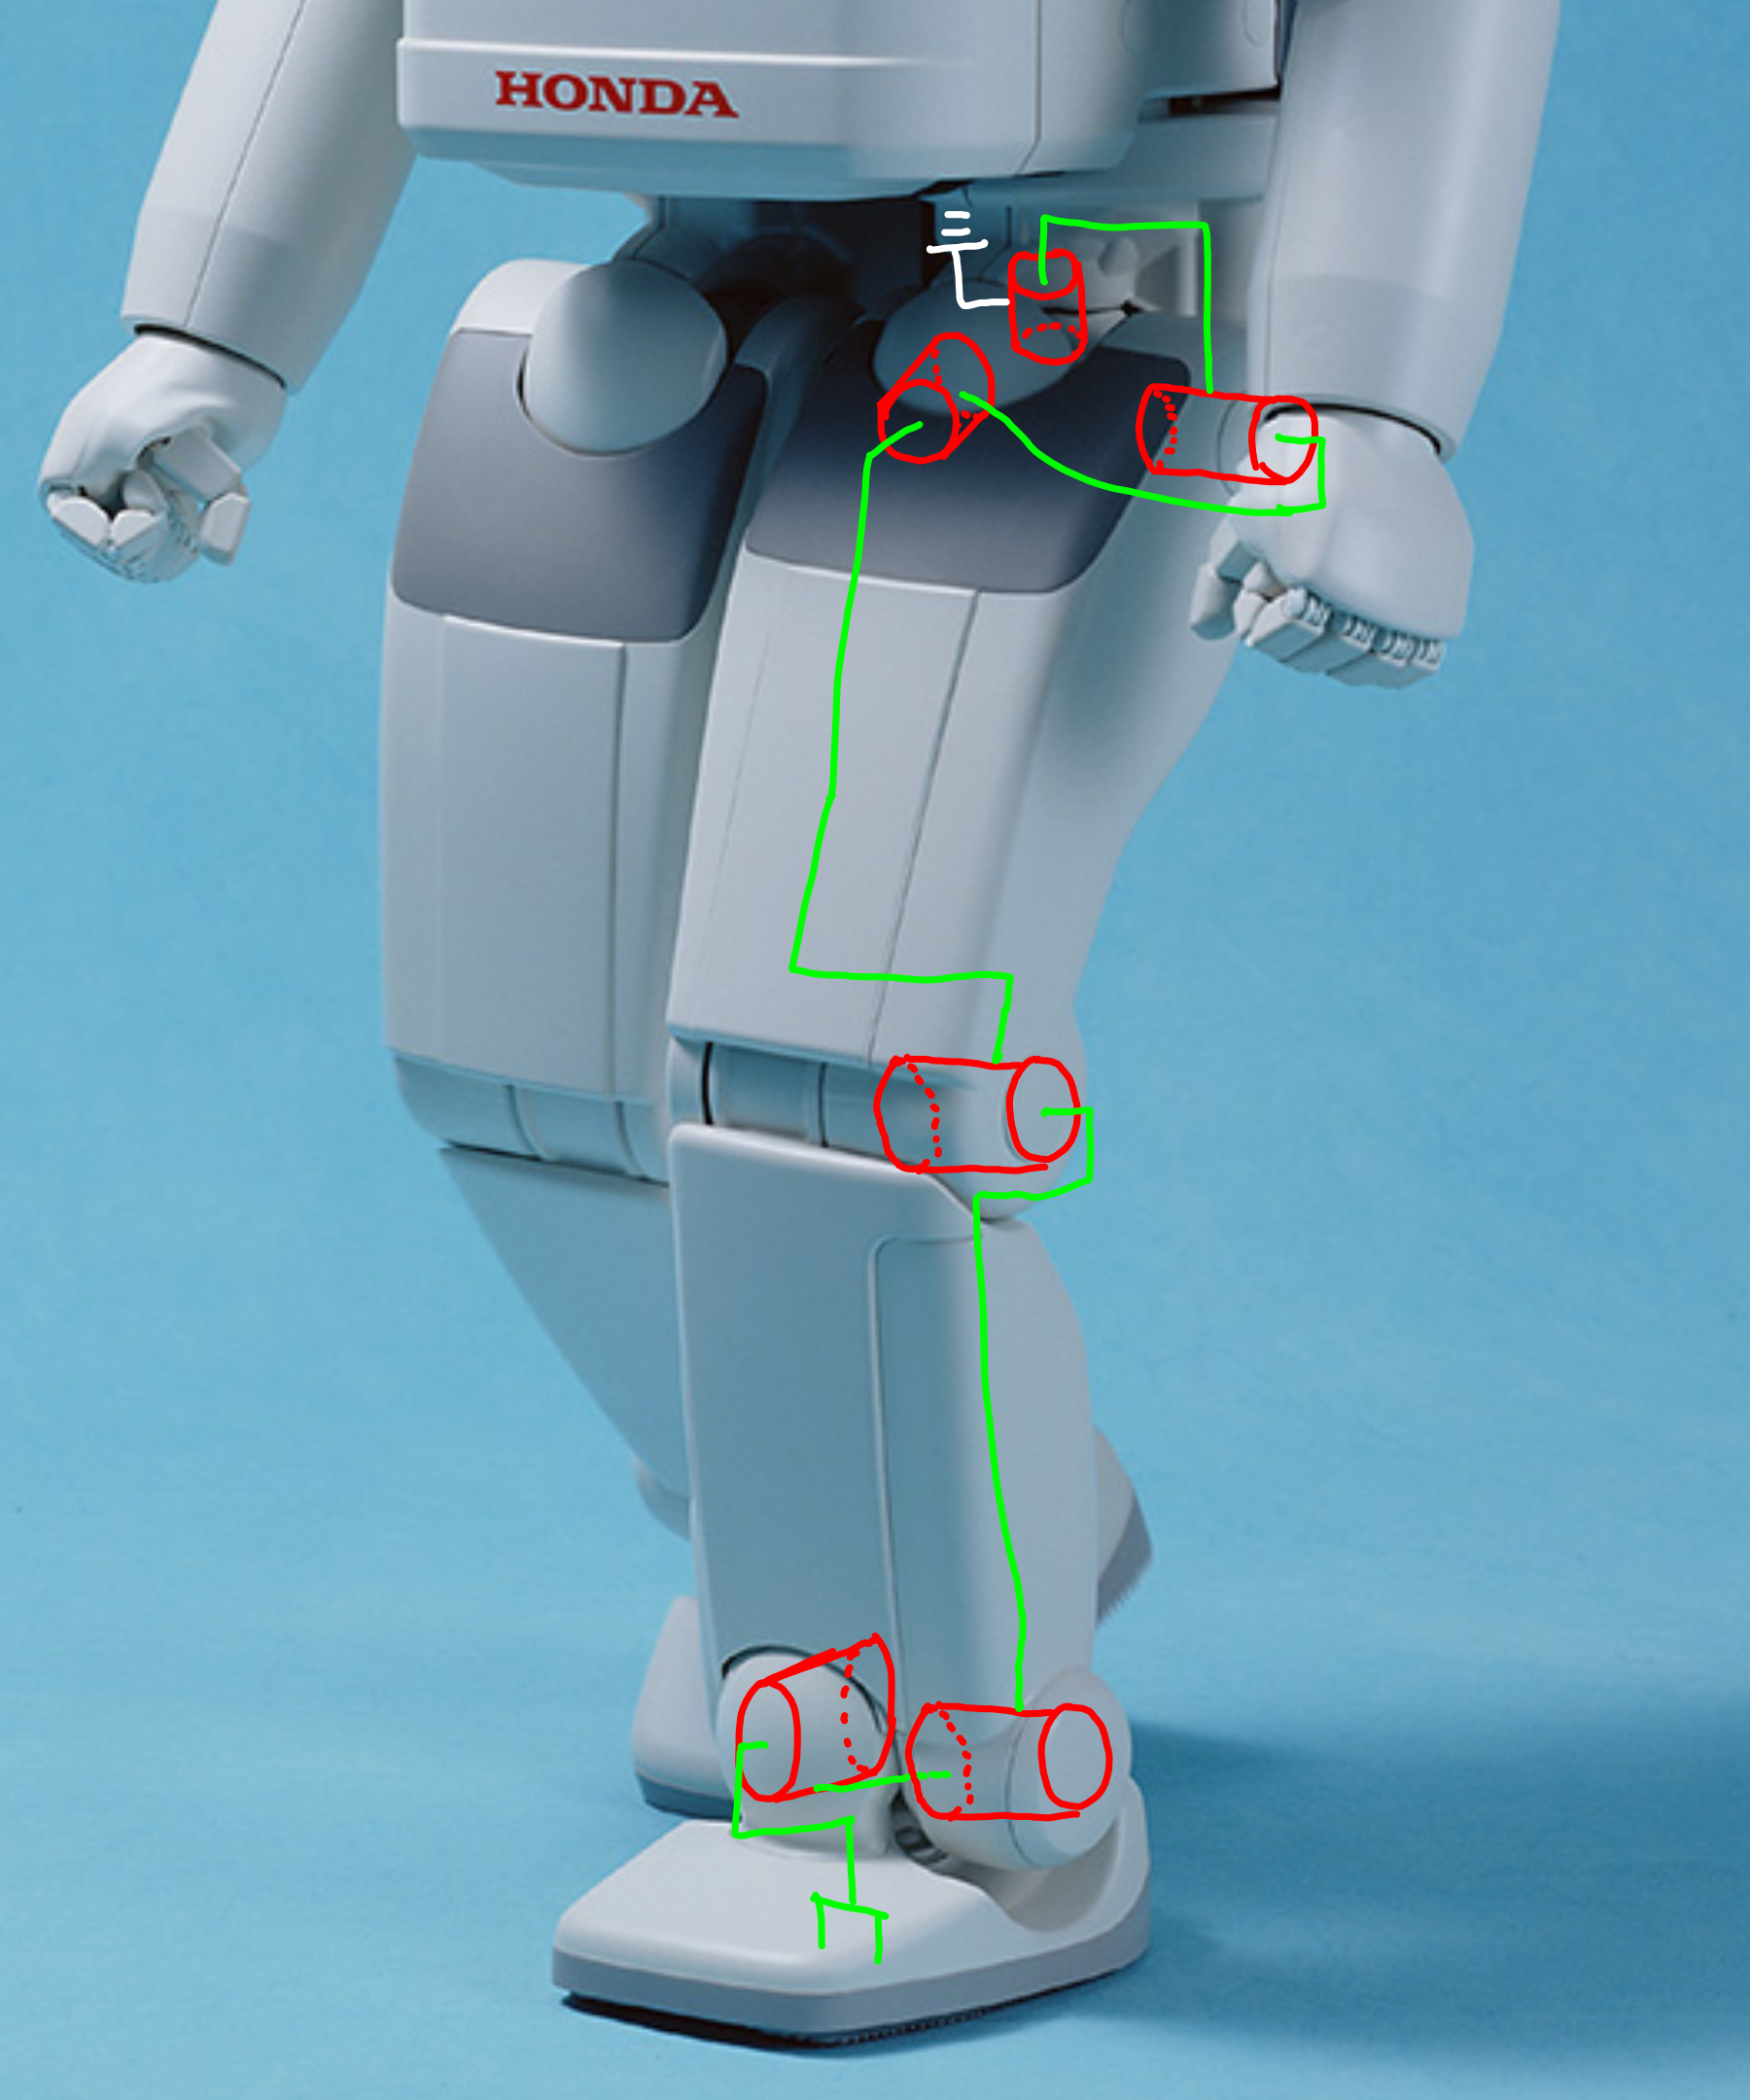
\includegraphics[width=.9\linewidth]{asimo.png}
\end{center}

\appendix
\section{\texttt{rotmat2axisangle.m}}
\label{sec:org7748d54}
\label{appendix:source}

\begin{minted}[]{matlab}
function [s, theta] = rotmat2axisangle(Q)

    lambdas = eig(Q);
    % Get eigenvalue with positive imaginary part
    thetas = imag(log(lambdas));
    theta = thetas(thetas > 0);

    sx = logm(Q)/theta;

    s = [sx(3, 2); -sx(3, 1); sx(2, 1)];
end
\end{minted}
\end{document}